\documentclass[a4paper,12pt]{article}

\usepackage[
    left=2cm,
    right=2cm,
    top=3cm,
    bottom=3cm
]{geometry}

\usepackage[utf8]{inputenc}
\usepackage[czech]{babel}
\usepackage[T1]{fontenc}
\usepackage{graphicx}
\usepackage{array}
\usepackage{booktabs}
\usepackage{tabularx}
\usepackage{makecell}
\usepackage{float}
\usepackage{newunicodechar}
\usepackage{url}
\usepackage{siunitx}
\usepackage{listings}
\usepackage{gensymb}
\usepackage{amsmath}
\usepackage{xcolor}
\usepackage{diagbox}
\usepackage{hyperref}
\usepackage{tikz}
\usepackage{pgfplots}
\pgfplotsset{compat=1.18}

\usepackage{fancyhdr}
\pagestyle{fancy}

\fancyhf{}
\fancyhead[L]{SME -- Lab 3: Měření na spínaném obvodu}
\fancyhead[R]{Pavel Pernička}
\fancyfoot[C]{\thepage}

\fancypagestyle{firstpage}{
    \fancyhf{}
    \renewcommand{\headrulewidth}{0pt}
    \renewcommand{\footrulewidth}{0pt}
    \fancyfoot[C]{\thepage}
}

\definecolor{myblue}{RGB}{111,0,248}
\newcommand{\colorcircle}[1]{%
  \tikz[baseline=-0.6ex]\draw[fill=#1,draw=none] (0,0) circle (1.5ex);%
}
\newcommand{\unitC}{\,^\circ\mathrm{C}}
\newcommand{\unitV}{\,\mathrm{V}}
\newcommand{\unitA}{\,\mathrm{A}}
\newcommand{\units}{\,\mathrm{s}}
\newcommand{\unitmin}{\,\mathrm{min}}

\newcommand{\centered}[1]{\begin{tabular}{l} #1 \end{tabular}}

\addto\captionsczech{\renewcommand{\refname}{Seznam použité literatury}}
\addto\captionsczech{\renewcommand{\figurename}{\textbf{Obrázek}}}
\addto\captionsczech{\renewcommand{\tablename}{\textbf{Tabulka}}}
\renewcommand{\lstlistingname}{\textbf{Kód}}

\lstset{
    language=Python,
    basicstyle=\ttfamily\footnotesize,
    keywordstyle=\color{blue},
    commentstyle=\color{gray},
    stringstyle=\color{red},
    numbers=left,
    numberstyle=\tiny\color{gray},
    stepnumber=1,
    breaklines=true,
    frame=single
}

\begin{document}
\thispagestyle{firstpage}

\vspace*{\fill}
\begin{center}
\renewcommand{\arraystretch}{1.75}

\begin{tabularx}{\textwidth}{|X|X|X|}
    \hline
    \multicolumn{1}{|c|}{\rule{0pt}{2.25cm} 
\includegraphics[height=2cm]{img/ctu_logo.png}}
    & \multicolumn{2}{c|}{\makecell{\textbf{KATEDRA MĚŘENÍ}}} \\
    \hline
    \multicolumn{3}{|c|}{\Large \textbf{\centered{Senzory a měření}}} \\
    \hline
    \multicolumn{2}{|X}{\small{Jméno} \newline \textbf{Pavel Pernička}}
    & \multicolumn{1}{|X|}{\small{Datum měření} \newline \textbf{25.3.2026}} \\
    \hline
    {\small{Semestr} \newline \textbf{Letní 2026}}
    & {\small{Ročník} \newline \textbf{2.}}
    & {\small{Datum odevzdání} \newline \textbf{1.4.2026}} \\
    \hline
    \multicolumn{3}{|c|}{\rule{0pt}{1cm}} \\
    \hline
    \multicolumn{1}{|X|}{\small{Číslo úlohy \newline \textbf{3}}}
    & \multicolumn{2}{|p{9cm}|}{\small{Název úlohy \newline \textbf{Měření na spínaném obvodu}}} \\
    \hline
\end{tabularx}

\end{center}
\vspace*{\fill}

\newpage
\pagestyle{fancy}
\section{Domácí příprava}
\begin{itemize}
  \item Co znamená zkratka RMS (popř. True RMS) u funkce střídavých měření napětí a proudu?
    \begin{itemize}
      \item Root mean square, což nám přímo říká, jakým způsoben se počítá efektivní hodnota:
      $$
        U_{\mathrm{RMS}} = \sqrt{\frac{1}{T} \int_0^T u^2(t)\,\mathrm{d}t}
      $$
    \end{itemize}
  \item Jakou hodnotu měří většina číslicových multimetrů, které tuto zkratku u funkce střídavých měření napětí a proudu nemají?
    \begin{itemize}
      \item Aritmetickou střední hodnotu přenásobenou konstantou $k = 1,11$ pro sinusový průběh. To bude dělat problém, když průběh sinusový nebude.
    \end{itemize}
  \item Lze těmito multimetry měřit efektivní hodnotu při nesinusovém průběhu napětí popř. proudu? Lze v tomto případě určit střední hodnotu? Pokud ano, jak?
    \begin{itemize}
      \item Nelze, protože vynásobení konstantou $1,11$ dává smysluplnou hodnotu jen pro sinusový průběh. Střední hodnotu v pravém slova smyslu také nezískáme, protože tento typ voltmetru pracuje pouze s absolutními hodnotami proudu/napětí. Dokážeme získat pouze aritmetickou střední hodnotu -- a to vydělením tou konstantou.
    \end{itemize}
\end{itemize}

\section{Měření}
Pro měření byly použity tyto přístroje:
\begin{itemize}
  \item $V_1$ \dots Summit 45
  \item $V_2$ \dots Agilent 34401A
  \item $V_3$ \dots Keysight U1241C
  \item Osciloskop \dots Keysight MSO-X 3012T, s děličem 1:4
\end{itemize}
\subsection{Napětí na zátěži při různých úhlech sepnutí}
Změřte napětí na zátěži, jejíž výkon je regulován obvodem s triakem pro úhel sepnutí $\alpha$ přibližně 0°, 45° a 90° předloženými číslicovými multimetry V1 až V3.
Průběh napětí sledujte na osciloskopu (osciloskop připojte na výstup odporového děliče). Efektivní a střední hodnotu změřte pomocí automatických měřicích funkcí osciloskopu.
\par\noindent\rule{\textwidth}{0.4pt}

\begin{table}[H]
\centering
\begin{tabular}{|c|c|c|c|}
\hline
 & $\mathbf{0^\circ}$ & $\mathbf{45^\circ}$ & $\mathbf{90^\circ}$ \\
\hline
$\mathbf{V_1}$ & $36,53\ V$ & $31,56\ V$ & $19,14\ V$ \\
\hline
$\mathbf{V_2}$ & $36,87\ V$ & $34,97\ V$ & $26,58\ V$ \\
\hline
$\mathbf{V_3}$ & $37,02\ V$ & $35,30\ V$ & $26,28\ V$ \\
\hline
\end{tabular}
\caption{Napětí na zátěži pomocí voltmetrů}
\end{table}

\begin{table}[H]
\centering
\begin{tabular}{|c|c|c|c|}
\hline
 & $\mathbf{0^\circ}$ & $\mathbf{45^\circ}$ & $\mathbf{90^\circ}$ \\
\hline
$\mathbf{V_{RMS}}$ & $7,44\ V$ & $7,115\ V$ & $5,354\ V$ \\
\hline
$\mathbf{V_{AVG}}$ & $-184\ mV$ & $-169\ mV$ & $-162\ mV$ \\
\hline
\end{tabular}
\caption{Efektivní a střední hodnota napětí pomocí osciloskopu}
\end{table}

\begin{table}[H]
\centering
\begin{tabular}{|c|c|c|c|}
\hline
 & $\mathbf{0^\circ}$ & $\mathbf{45^\circ}$ & $\mathbf{90^\circ}$ \\
\hline
$\mathbf{V_{RMS}}$ & $37{,}20\ \mathrm{V}$ & $35{,}58\ \mathrm{V}$ & $26{,}77\ \mathrm{V}$ \\
\hline
$\mathbf{V_{AVG}}$ & $-920\ \mathrm{mV}$ & $-845\ \mathrm{mV}$ & $-810\ \mathrm{mV}$ \\
\hline
\end{tabular}
\caption{Přepočtené hodnoty z osciloskopu podle děliče}
\end{table}

\subsection{Správná efektivní hodnota}
Určete, které z multimetrů měří správně efektivní hodnotu, a určete relativní chybu metody měření efektivní hodnoty u ostatních.
\par\noindent\rule{\textwidth}{0.4pt}
Správně efektivní hodnotu měří $V_2$ (Agilent 34401A) a $V_3$ (Keysight U1241C). Multimetr $V_1$ (Summit 45) měří aritmetickou střední hodnotu přenásobenou konstantou pro sinusový průběh, a proto při průběhu s uříznutým sinem vykazuje chybu. 
Jako referenční hodnoty byly použity hodnoty změřené osciloskopem:
$$
\delta = \frac{|V_x - V_{\mathrm{ref}}|}{V_{\mathrm{ref}}}\cdot 100\,\%.
$$
Pro jednotlivé úhly vyšla následovně: $0^\circ$ rovna $1{,}80\,\%$, při $45^\circ$ rovna $11{,}30\,\%$ a při $90^\circ$ rovna $28{,}50\,\%$. Je vidět, že s rostoucí deformací průběhu se chyba výrazně zvětšuje.

\subsection{Střední hodnota}
Z údaje multimetrů, které to umožňují, určete střední hodnotu měřeného průběhu.
\par\noindent\rule{\textwidth}{0.4pt}

Z non-RMS voltmetru $V_1$ jsme schopni získat jen aritmetickou střední hodnotu:
$$
U_{str} = \frac{U_{measured}}{1,11}
$$

\begin{table}[H]
\centering
\begin{tabular}{|c|c|c|c|}
\hline
 & $\mathbf{0^\circ}$ & $\mathbf{45^\circ}$ & $\mathbf{90^\circ}$ \\
\hline
$\mathbf{V_{str}}$ & $32{,}91\ \mathrm{V}$ & $28{,}43\ \mathrm{V}$ & $17{,}24\ \mathrm{V}$ \\
\hline
\end{tabular}
\caption{Střední aritmetická hodnota napětí vypočtená z $V_1$}
\end{table}

U true-RMS přístrojů ztratíme znaménko kvůli kvadrátu v definici, proto jsme rovněž schopni přepočítat jen střední aritmetickou hodnotu.
Pro úhel sepnutí $0^\circ$ lze předpokládat sinusový průběh, a tedy použít vztah
$$
V_{\mathrm{str}} = \frac{2\sqrt{2}}{\pi} \, V_{\mathrm{ef}}.
$$

Z toho vychází:
$$
\begin{aligned}
V_2: \quad & V_{\mathrm{str}} \approx 33{,}18\ \mathrm{V}, \\
V_3: \quad & V_{\mathrm{str}} \approx 33{,}32\ \mathrm{V}.
\end{aligned}
$$

\subsection{Výpočet stř. a ef. hodnoty z definic}
Pro úhel sepnutí $\alpha = 90\degree$ určete aritmetickou střední hodnotu a efektivní hodnotu napětí rovněž výpočtem z definic (maximální hodnotu určete z údaje nejpřesnějšího z multimetrů při $\alpha = 0\degree$).
Vypočtené hodnoty porovnejte s naměřenými a v případě rozdílu analyzujte možné příčiny.
\par\noindent\rule{\textwidth}{0.4pt}
Jako nejpřesnější byl zvolen multimetr $V_2$, který při $\alpha = 0^\circ$ naměřil efektivní hodnotu
$$
U_{\mathrm{eff}} = 36{,}87\ \mathrm{V}.
$$

Při úhlu sepnutí $\alpha = 0^\circ$ je průběh sinusový, proto lze maximální hodnotu určit ze vztahu mezi efektivní hodnotou a amplitudou sinusového průběhu:
$$
U_{\mathrm{eff}} = \frac{U_{max}}{\sqrt{2}},
$$
odkud
$$
U_{max} = \sqrt{2}\,U_{\mathrm{eff}} = \sqrt{2}\cdot 36{,}87 \approx 52{,}14\ \mathrm{V}.
$$

Pro úhel sepnutí $\alpha = 90^\circ = \frac{\pi}{2}$ je triak sepnut pouze v intervalech
$$
\left\langle \frac{\pi}{2}, \pi \right\rangle
\quad \text{a} \quad
\left\langle \frac{3\pi}{2}, 2\pi \right\rangle.
$$

Pro aritmetickou střední hodnotu:
$$
U_{str} = \frac{1}{T}\int_0^T |u(t)|\,dt.
$$

Díky symetrii můžeme zjednodušit:
$$
U_{str} = \frac{1}{2\pi}\left( 2\int_{\pi/2}^{\pi} U_{max}\sin\varphi\,d\varphi \right).
$$
$$
U_{str} = \frac{U_{max}}{\pi}\int_{\pi/2}^{\pi}\sin\varphi\,d\varphi.
$$
$$
\int_{\pi/2}^{\pi}\sin\varphi\,d\varphi
=
[-\cos\varphi]_{\pi/2}^{\pi}
=
(-\cos\pi)-(-\cos\frac{\pi}{2})
= 1.
$$

Proto
$$
U_{str} = \frac{U_{max}}{\pi} = \frac{52{,}14}{\pi} \approx 16{,}60\ \mathrm{V}.
$$

Efektivní hodnota se určí z definice
$$
U_{\mathrm{ef}} = \sqrt{\frac{1}{T}\int_0^T u^2(t)\,dt}.
$$

Opět využijeme symetrii:
$$
U_{\mathrm{ef}} =
\sqrt{
\frac{1}{2\pi}
\left(
2\int_{\pi/2}^{\pi} U_{max}^2\sin^2\varphi\,d\varphi
\right)
}.
$$
$$
U_{\mathrm{ef}} =
U_{max}\sqrt{
\frac{1}{\pi}\int_{\pi/2}^{\pi}\sin^2\varphi\,d\varphi
}.
$$
Dosadíme:
$$
\int_{\pi/2}^{\pi}\sin^2\varphi\,d\varphi
=
\left[\frac{\varphi}{2} - \frac{\sin(2\varphi)}{4}\right]_{\pi/2}^{\pi}
=
\frac{\pi}{2} - \frac{\pi}{4}
=
\frac{\pi}{4}.
$$

A získáme:
$$
U_{\mathrm{ef}} =
U_{max}\sqrt{\frac{1}{\pi}\cdot\frac{\pi}{4}}
=
\frac{U_{max}}{2}
=
\frac{52{,}14}{2}
\approx 26{,}07\ \mathrm{V}.
$$

Výpočtem tedy pro $\alpha = 90^\circ$ vychází:
$$
U_{str} \approx 16{,}60\ \mathrm{V},
\qquad
U_{\mathrm{ef}} \approx 26{,}07\ \mathrm{V}.
$$

Vypočtená efektivní hodnota odpovídá hodnotám naměřeným true-RMS multimetry. Aritmetická střední hodnota také přibližně odpovídá hodnotě určené z non-True RMS voltmetru.

\subsection{Měření při různých frekvencích}
Připojte multimetry ke generátoru programovatelných průběhů. Proveďte měření sinusového průběhu -- napětí o efektivní hodnotě $0,7\ V$ při frekvencích $10\ Hz$, $100\ Hz$, $1\ kHz$, $10\ kHz$, $100\ kHz$ a $1\ MHz$.
\par\noindent\rule{\textwidth}{0.4pt}

\begin{table}[H]
\centering
\begin{tabular}{|c|c|c|c|c|c|c|}
\hline
 & $\mathbf{10\ Hz}$ & $\mathbf{100\ Hz}$ & $\mathbf{1\ kHz}$ & $\mathbf{10\ kHz}$ & $\mathbf{100\ kHz}$ & $\mathbf{1\ MHz}$ \\
\hline
$\mathbf{V_1}$ & $0{,}713\ \mathrm{V}$ & $0{,}707\ \mathrm{V}$ & $0{,}696\ \mathrm{V}$ & $0{,}35\ \mathrm{V}$ & $0{,}001\ \mathrm{V}$ & $0\ \mathrm{V}$ \\
\hline
$\mathbf{V_2}$ & $0{,}708\ \mathrm{V}$ & $0{,}711\ \mathrm{V}$ & $0{,}712\ \mathrm{V}$ & $0{,}712\ \mathrm{V}$ & $0{,}710\ \mathrm{V}$ & $0{,}727\ \mathrm{V}$ \\
\hline
$\mathbf{V_3}$ & $0{,}703\ \mathrm{V}$ & $0{,}713\ \mathrm{V}$ & $0{,}713\ \mathrm{V}$ & $0{,}715\ \mathrm{V}$ & $0{,}734\ \mathrm{V}$ & $0\ \mathrm{V}$ \\
\hline
\end{tabular}
\caption{Závislost naměřeného napětí na frekvenci signálu}
\end{table}

\subsection{FFT}
Připojte generátor přímo k osciloskopu. Na generátoru nastavte postupně průběh obdélníkový, sinusový a trojúhelníkový, frekvenci $100\ kHz$, rozkmit $1\ V_{šš}$. Při obdélníkovém průběhu určete vliv počtu bodů pro
výpočet FFT a nastavení počtu zobrazených period. Změřená spektra si poznamenejte (orientační údaje o
frekvenci harmonických a jejich amplitudě). Jak se liší zobrazení FFT pro nastavení vertikálních
jednotek $V_{rms}$ a $dB$?

\par\noindent\rule{\textwidth}{0.4pt}

Na obrázcích jsou zachycena spetra pro různé tvary vstupního signálu. U sinusového vidíme ve středu jednu hlavní frekvenci $100\ kHz$, u trojúhelníkového a obdélníkového vidíme nalevo hlavní frekevnci a liché harmonické, přičemž u trojúhelníku klesá amplituda harmonických frekvencí výrazně rychleji, než u obdélníku.  V obou případech také vidíme ve spektru různé mezifrekvence, které vznikly pravděpodobně v důsledku spektrálního prosakování nebo spíše méně pravděpodobně v důsledku vysokofrekvenčního šumu. 

Jak jde vidět při srovnání obrázků \ref{fig:char3} a \ref{fig:char4}, zvýšení počtu bodů, ze kterých se FFT počítá vede k ostřejším peakům ve spektru. 

V našem případě používéme logaritmickou škálu ($dB$) zobrazení aplitud, protože nám umožňuje lépe pozorovat i menší peaky a jednodušeji porovnávat jejich velikosti.

\begin{figure}[H]
\centering
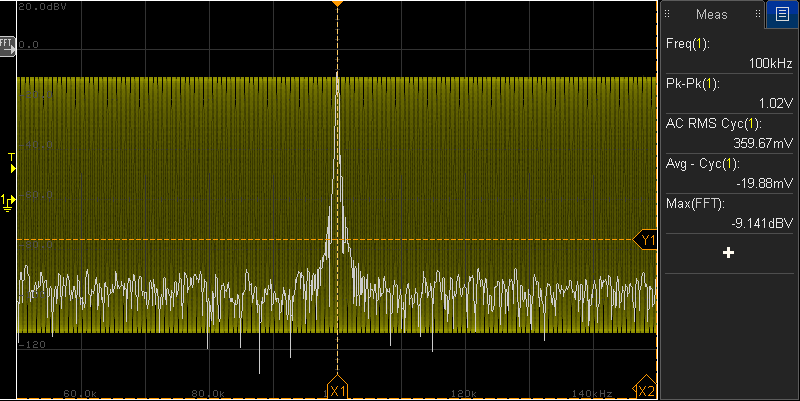
\includegraphics[width=0.95\textwidth]{img/scope_4.png}
\caption{Spektrum sinusového průběhu}
\label{fig:char1}
\end{figure}

\begin{figure}[H]
\centering
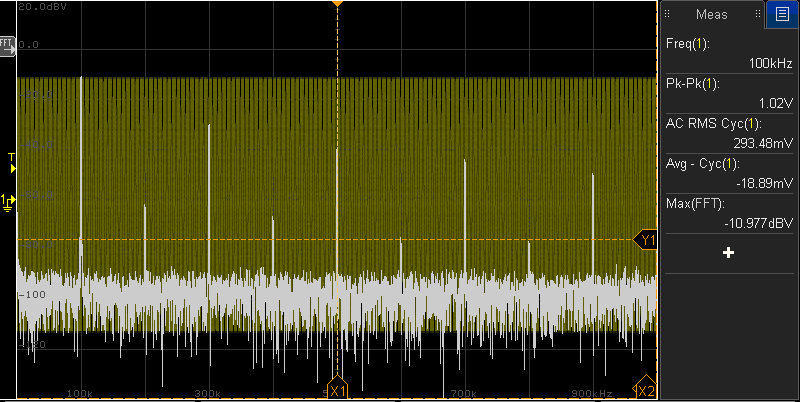
\includegraphics[width=0.95\textwidth]{img/scope_5.png}
\caption{Spektrum trojúhelníkového průběhu}
\label{fig:char2}
\end{figure}

\begin{figure}[H]
\centering
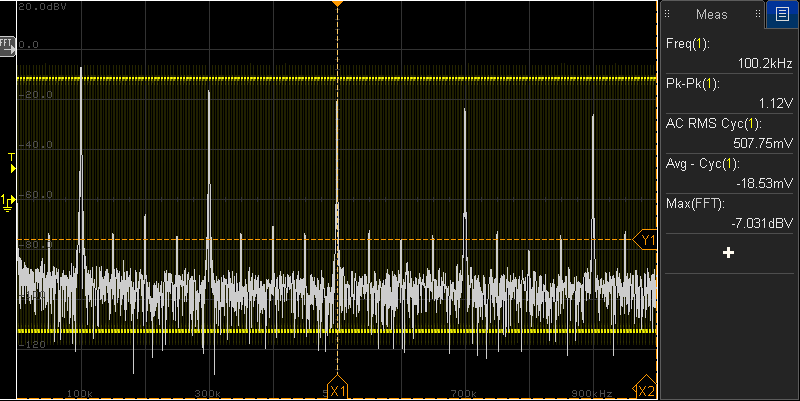
\includegraphics[width=0.95\textwidth]{img/scope_6.png}
\caption{Spektrum obdélníkového průběhu s větším počtem bodů}
\label{fig:char3}
\end{figure}

\begin{figure}[H]
\centering
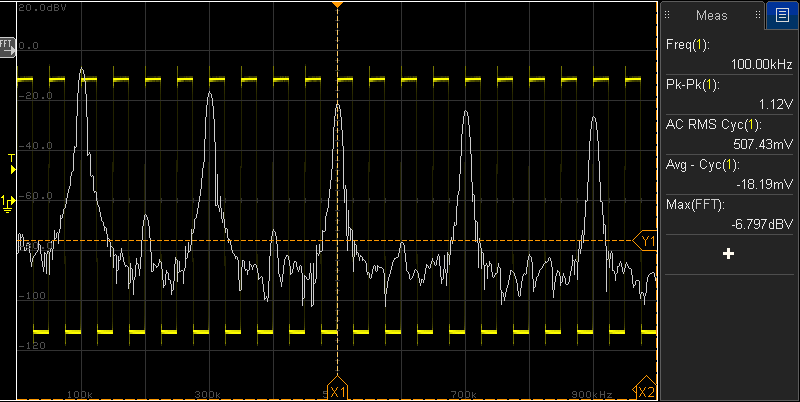
\includegraphics[width=0.95\textwidth]{img/scope_7.png}
\caption{Spektrum obdélníkového průběhu s menším počtem bodů}
\label{fig:char4}
\end{figure}

\end{document}
